\subsection{MSVC + \olly}
\myindex{\olly}
Illustriamo il funzionamento con \olly.
Quando raggiungiamo la prima istruzione in \ttf che usa uno degli argomenti (il primo) 
notiamo che \EBP punta allo \gls{stack frame}, indentificato dal riquadro rosso.

Il primo elemento dello \gls{stack frame} e' il valore salvato di \EBP, 
il secondo e' il \ac{RA}, il terzo rappresenta il primo argomento della funzione, seguito dal secondo e terzo argomento.

Per accedere al primo argomento della funzione bisogna aggiungere esattamente 8 (2 word a 32-bit) a \EBP.

\olly e' in grado di distinguere gli argomenti in quesot modo, ed ha aggiunto dei commenti agli elementi dello stack, ad esempio:

\q{RETURN from} and \q{Arg1 = \dots}, etc.

N.B.: Gli argomenti della funzione non sono membri dello stack frame della funzione chiamata, appartengono allo stack frame della
funzione chiamante (\gls{caller}).

Pertanto \olly ha contrassegnato gli elementi \q{Arg} come membri di un altro stack frame.

\begin{figure}[H]
\centering
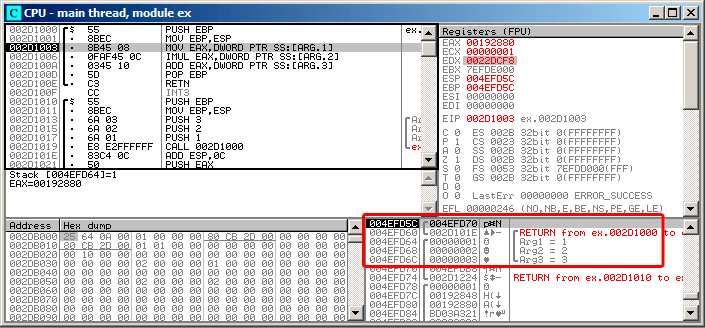
\includegraphics[scale=\FigScale]{patterns/05_passing_arguments/olly.png}
\caption{\olly: inside of \ttf{} function}
\label{fig:passing_arguments_olly}
\end{figure}
